\documentclass[a4paper, 11pt]{article}
\usepackage{comment} % enables the use of multi-line comments (\ifx \fi)  
\usepackage{fullpage} % changes the margin
\usepackage{mathtools} %allows us to write complex equations
\usepackage{graphicx} %allows us to add pictures
\usepackage{amsmath} %allows us to add Greek letters and equations
\usepackage{float} %formatting pictures
\usepackage{afterpage}
\usepackage{tikz}
\usetikzlibrary{automata, positioning, arrows}
\tikzset{->,>=stealth',node distance=3cm}

\begin{document}
\noindent
\large\textbf{Homework 1} \hfill \\
\large{Mike Gao} \\
\normalsize 260915701 \\
Prof. Prakash Panangaden \hfill 


\section*{Question 1}
We have $f:\Sigma \rightarrow M$ and want $f^*:\Sigma^* \rightarrow M$ to be a homomorphism.

First we define $\Sigma^* = \Sigma_0 \cup \Sigma_1 \cup ...$ where $\Sigma_k $ is the set containing words of length k

We define $f^*$ on $\Sigma_0$ be the map to identity element. $f^*(\epsilon)= \epsilon$, on $\Sigma_1$ as equal to the element in $\Sigma$ such that $\forall e \in \Sigma: f^*(e) = f(e)$, and on $\Sigma_{i+1}$ given $mn\in\Sigma_{i+1}$ where $m\in\Sigma_i$ and $n\in\Sigma$ we define $f^*(mn)=f^*(m)f(n)$

In order to prove $f^*$ is a monoid homomorphism, we show that the identity element is preserved $f^*(\epsilon) = \epsilon$ by definition.
We also need to prove the binary operations is preserved. Let $\star$ be the binary operation on M and $\circ$ be the binary operation on $\Sigma^*$.Let $ai, bi \in \Sigma$

$f^*(x)\star f^*(y) = (f(a_1)\star f(a_2) \star f(a_3) \star \cdots \star f(a_n))\star (f(b_1)\star f(b_2) \star f(b_3) \star \cdots \star f(b_n))$ 

$= f(a_1)\star f(a_2) \star f(a_3) \star \cdots \star f(a_n) \star (f(b_1)\star f(b_2) \star f(b_3) \star \cdots \star f(b_n)$ by associativity

$=f^*(a_1\circ a_2 \circ a_3 \circ \cdots b_n)$

$=f^*(x\circ y)$

In order to prove uniqueness, we can do it with induction. Any other $g$ which agree with $f^*$ on $\Sigma_i$ will agree on $\Sigma_{i+1}$ since $g(xy)=g(x)f(y)=f^*(x)f(y)=f^*(xy)$



\section*{Question 2}
($\rightarrow$)Let $A=(Q, A, i, \delta, T)$ be a DFA such that it recognizes L and let $T(A)$ be the transition monoid of A. Let $f: A^* \rightarrow T(A)$ the function associating the string with the effect of the string on the set Q. Let $I=f(L)$ be the image of the language in the transition monoid. Clearly, $L \subseteq f^-1(I)$ Let $x \in f^-1(I)$, Then by definition there exist an $y \in L$ such that $f(x) = f(y)$. But $y \in L(A)$ and so $x \in L(A)$ hence $x \in L$

\noindent($\leftarrow$)Proving the converse: Suppose that L is recognized by a finite monoid. There is a monoid homomorphism $f:A^*\rightarrow{M}$ and a subset $S\subseteq{M}$ such that $L=f^{-1}(S)$. Define $A = \{M,A,i,\delta,S\}$ where i is the identity of M and $\delta(p,q) = p\circ f(q)$ It is clear that A is a finite automaton. If q is a string that is in $A^*$ then $\delta^*(p,q) = p\circ f(q)$ We have that $x\in{L(A)}$ if and only if $i\circ f(x)\in{S}$ if and only if $x\in{f^{-1}(S)}$ which is L. So L(A) = L

\section*{Question 3}
Suppose h is not inflationary, i.e. $V= \{x | x > h(x)\}$ and V not emptyset. W is well-founded so that V has minimal element such that $v_0 > h(v_0)$. Since $\forall y < v_0$, $y\leq{h(y)}$, we have $h(v_0)\leq{h(h(v_0))}$. However, since h is strictly monotone, we can deduce $h(v_0)\geq{h(h(v_0))}$ from $v_0\geq{h(v_0)}$ Thus an contradiction is found.

\section*{Question 4}
\subsection*{4.1}
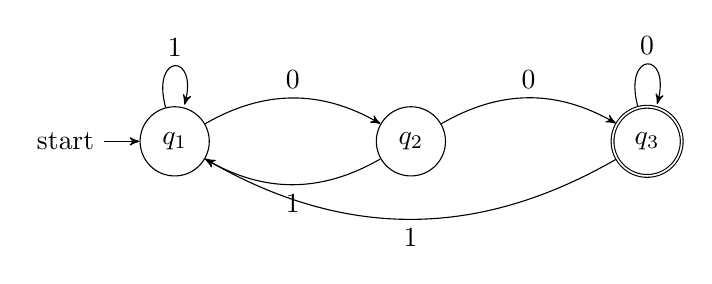
\begin{tikzpicture}
\node[state, initial] (q1) {$q_1$};
\node[state, right of=q1] (q2) {$q_2$};
\node[state, accepting, right of=q2] (q3) {$q_3$};
\draw (q1) edge[loop above] node{1} (q1)
(q1) edge[bend left, above] node{0} (q2)
(q2) edge[bend left, below] node{1} (q1)
(q2) edge[bend left, above] node{0} (q3)
(q3) edge[loop above] node{0} (q3)
(q3) edge[bend left, below] node{1} (q1);
\end{tikzpicture}
\subsection*{4.2}
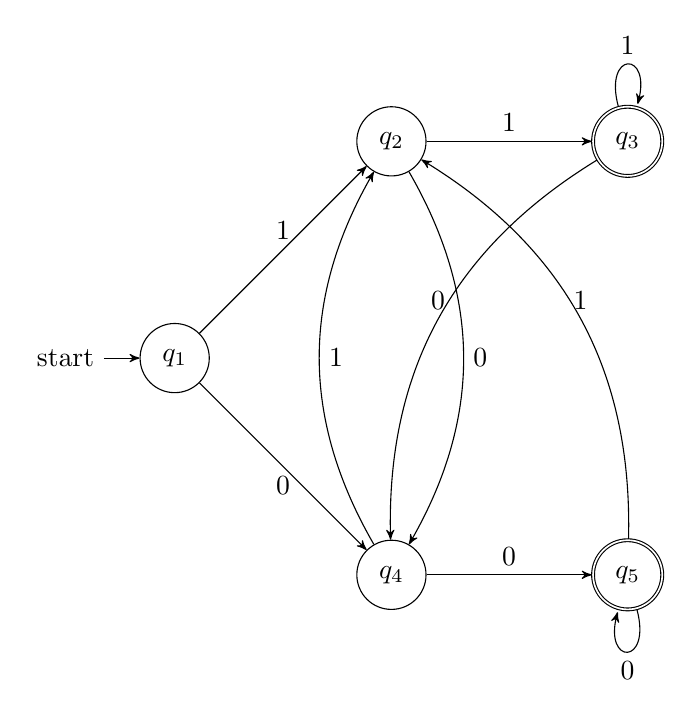
\begin{tikzpicture}
\node[state, initial] (q1) {$q_1$};
\node[state, above right=of q1] (q2) {$q_2$};
\node[state, below right=of q1] (q4) {$q_4$};
\node[state, accepting, right of = q4] (q5) {$q_5$};
\node[state, accepting, right of = q2] (q3) {$q_3$};

\draw 
(q1) edge[above] node{1} (q2)
(q1) edge[below] node{0} (q4)
(q2) edge[above] node{1} (q3)
(q3) edge[loop above] node{1} (q3)
(q5) edge[loop below] node{0} (q5)
(q3) edge[bend right, above] node{0} (q4)
(q5) edge[bend right, above] node{1} (q2)
(q2) edge[bend left, right] node{0} (q4)
(q4) edge[bend left, right] node{1} (q2)
(q4) edge[above] node{0} (q5);
\end{tikzpicture}
\subsection*{4.3}
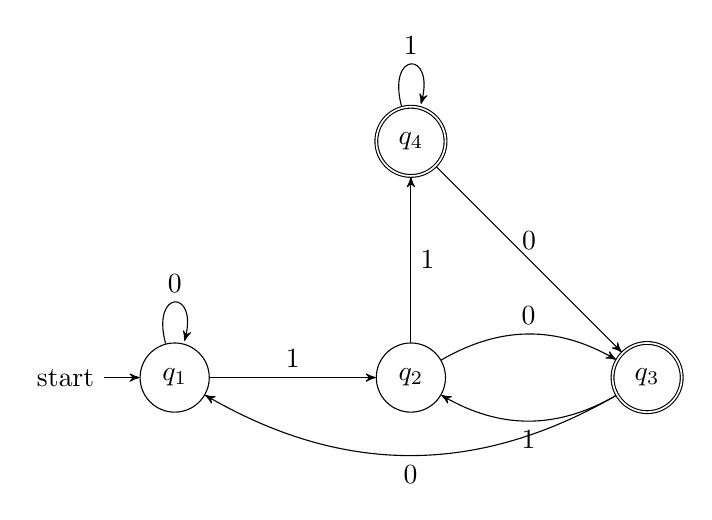
\begin{tikzpicture}
\node[state, initial] (q1) {$q_1$};
\node[state, right of=q1] (q2) {$q_2$};
\node[state, accepting, right of=q2] (q3) {$q_3$};
\node[state, accepting, above of=q2] (q4) {$q_4$};
\draw (q1) edge[loop above] node{0} (q1)
(q1) edge[above] node{1} (q2)
(q2) edge[right] node{1} (q4)
(q2) edge[bend left, above] node{0} (q3)
(q4) edge[loop above] node{1} (q4)
(q4) edge[above] node{0} (q3)
(q3) edge[bend left, below] node{1} (q2)
(q3) edge[bend left, below] node{0} (q1);
\end{tikzpicture}

\section*{Question 5}
We assume $(S,s_0,F,\delta)$ is a DFA that recognizes L.
We now construct a NFA $(Q,Q_0,F,\Delta)$ for middle($L$).



  $Q = \overbrace{S}^{\text{track } v}
  \times \underbrace{S}_{\mathclap{\substack{\text{guess where DFA will} \\ \text{be when $u$ ends}}}}
  \times \overbrace{S}^{\mathclap{\substack{\text{guess where DFA will} \\ \text{be when $v$ ends}}}}
  \times \underbrace{2^S}_{\text{track } u}
  \times \underbrace{2^S}_{\text{track } w}$
  
  $Q_0=\{(s,s,t,\{s_0\},\{t\})\}$
  
  $F' = \{ (t,s,t,X,Y) | Y'\cup F \neq \emptyset, s\in X\}$
  
  $\Delta ((s,s_c,t,X,Y),a) = (s',s_c,t,X',Y') $ where $\delta(s,a)=s'$, $X'$ and $Y'$ are the sets of states the DFA can reach from X and Y respectively reading any symbol

Since this is clearly a NFA that recognizes middle($L$), this is a regular language.

\section*{Question 6}
\subsection*{6.1}
\begin{tikzpicture}
\node[state, initial] (q0) {$q_0$};
\node[state, right of=q0] (q1) {$q_1$};
\node[state, right of=q1] (q2) {$q_2$};
\node[state, below right=of q2] (q3) {$q_3$};
\node[state, right of=q2] (q4) {$q_4$};
\draw 
(q0) edge[loop above] node{0} (q0)
(q0) edge[above] node{1} (q1)
(q1) edge[bend left, above] node{0} (q2)
(q2) edge[bend left, below] node{1} (q1)
(q2) edge[above] node{0} (q4)
(q3) edge[right] node{0} (q4)
(q1) edge[bend right, below] node{1} (q3)
(q3) edge[loop below] node{1} (q3)
(q4) edge[loop above, accepting] node{0,1} (q4);

\end{tikzpicture}
\subsection*{6.2}

Suppose that for contradiction we can find a correct DFA that has 4 states.

By the Pigeonhole Principle, if we choose 5 strings over $\Sigma$, then at least two of those strings must end at the same state q.

Let wi and wj be these 2 strings that satisfies the above.
For any string x, if wi and wj end at q, then wix and wjx must also end at the
same state r and hence must both be accepted or rejected by the DFA.
If we can pick for 5 strings such that, for any pair of them, for some x, that
wix is NOT in L (rejected) and wjx is in L (accepted), then we have a
contradiction, and what must assumed (we can find a correct DFA with 4
states) must be FALSE. 

We pick the following four strings

$W0 = \epsilon$

$W1 = 110$

$W2 = 010$

$W3 = 111$

$W4 = 101$

For one of the pairs of strings, the supposed 4-state DFA is forced into the same state for both strings (because of Pigeonhole principle), and $W_ix$ and $W_jx$ must be both accepted or rejected, for any string x. We will now show that for each pair this is NOT true.

Pair 1
Choose $x = \epsilon$

$W_0x = \epsilon$ reject $W_1x = 110$ accept

Pair 2
Choose $x = 0$

$W_0x = 0$ reject $W_2x = 0100$ accept

Pair 3
Choose $x = 10$

$W_0x = 10$ reject $W_3x = 11110$ accept

Pair 4
Choose $x = 10$

$W_0x = 10$ reject $W_4x = 10110$ accept

Pair 5
Choose $x = \epsilon$

$W_1x = 110$ accept $W_2x = 010$ reject

Pair 6
Choose $x = \epsilon$

$W_1x = 110$ accept $W_3x = 111$ reject

Pair 7
Choose $x = \epsilon$

$W_1x = 110$ accept $W_4x = 101$ reject

Pair 8
Choose $x = 10$

$W_2x = 01010$ reject $W_3x = 11110$ accept

Pair 9
Choose $x = 10$

$W_2x = 01010$ reject $W_4x = 10110$ accept

Pair 10
Choose $x = 0$

$W_3x = 1110$ accept $W_4x = 1010$ reject

A contradiction is found.

\section*{Question 7}

Assume $(S,s_0,F,\delta)$ is a DFA that recognizes L.
We know that a boolean matrix is finite and can be used in a NFA.
Let $M_{n*n}$ be a boolean matrix where $M_{ij}$ stores if NFA can get from $s_i$ to $s_j$ in $2^{|w|}$ steps where $|w|$ is the number of characters that has been read. So from M we can know if there exists a y such that $xy \in L$ and $|y| = 2^{|x|}$

Lets now construct an NFA $(Q,Q_0,F,\Delta)$

$Q = \underbrace{S}_{\text{track the state of the machine reading } x}
  \times \underbrace{S}_{\text{track where the machine will end up}} \times M$
  
$Q_0= \{(s_0, M)\}$

$F'= \{(s_i, M) | M_{ij} = 1 $ for $ s_j \in F\}$

$\Delta((s,M),a)=\{(\delta(s,a),M^2)\}$

This is clearly regular


\section*{Question 8}
\subsection*{8.1}
Demon pick $p > 0$ We choose $w=a^{2p}b^{p}$ such that $|w|>p$ always hold. Demon pick $y=a^{k}$, where $1\leq{k}\leq{p}$, I pick $i=0$, then $xy^{0}z=xz=a^{2p-k}b^{p}$
If $xy^{0}z\in{L}$, then $2p-k = 2p$ which means $k = 0$, but $k \leq {1}$ so we conclude that it is not regular.

\subsection*{8.2}
Demon pick $p > 0$. We choose $w=a^{(p+1)^2}$. In order to satisfy pumping lemma $|xy|\leq{p}$ and $|y|>0$, y need to consist exclusively with a. So $y=a^k$ for $0\leq{k}<p$. We then pick $i=2$, then new string $= xy^2z = a^{(p+1)^2+k}$ Since $(p+1)^2+k > (p+1)^2$ and $k\leq{p}$ we can then conclude that  $(p+1)^2+k\leq{(p+1)^2+p}<(p+2)^2$ and obviously $xy^2z \notin L$ So by pumping lemma it is not regular.

\section*{Question 9}

Proof by counterexample. Let $\Sigma = \{x,y,z\} $, $L = \{x^*zy^*\}$ Since L and ${x^*y^*}$ can be written as a regular expression, they are both regular. Now we need to prove outer(L) is not regular by showing $outer(L)\cap{\{x^*y^*\}}$ is not regular. 
Since there is no z in $\{x^*y^*\}$, for $uw\in{outer(L)\cap{\{x^*y^*\}}}$ there is no z in u or w, so z can only be in v
Since $L={x^*zy^*}$ and that z can only be in v, $u=x^*$ and $w=y^*$ and $v=x^*zy^*$ with $|u|=|w|=|v|$
So $u=x^n$, $w=y^n$ with some $n\geq{1}$
So $outer(L)\cap{\{x^*y^*\}} = \{x^*y^*,n\geq{1}\}$ 
Then, using pumping lemma to prove this is not regular.
Demon pick $p>0$, I choose $w=x^py^p$. Demon is forced to pick $ Y = x^k, k\geq1$ in order to satisfy $|XY| < p$ I choose i=2. Then $XY^iZ=x^{p+k}y^p\notin{\{x^ny^n | n\geq1\}}$
Since $outer(L)\cap{\{x^*y^*\}}$ is not regular, $outer(L)$ cannot be regular.


\section*{Question 10}
$\Sigma=\{1\}$
Build an NFA with nine states arranged in loops of length two and seven, Assign start and final state so that the shortest rejected string is of length $14 = 2 * 7$ and it is strictly greater than nine.

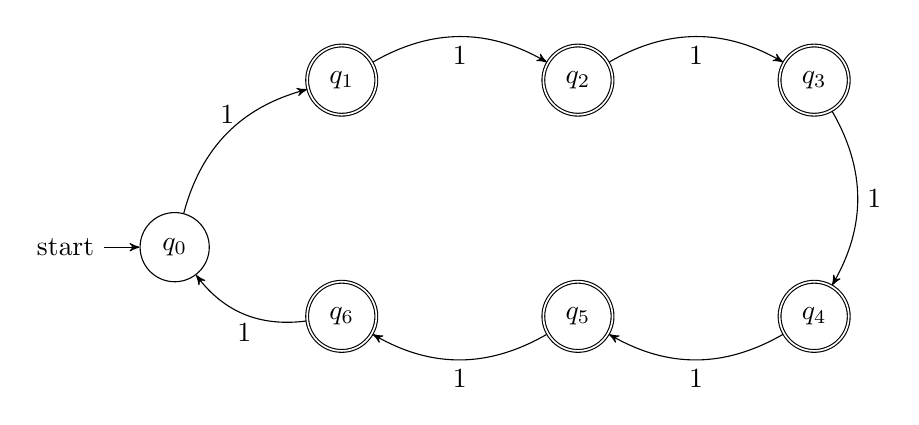
\begin{tikzpicture}
\node[state, initial] (q0) {$q_0$};
\node[state, accepting, above right of=q0] (q1) {$q_1$};
\node[state, accepting, right of=q1] (q2) {$q_2$};
\node[state, accepting, right of=q2] (q3) {$q_3$};
\node[state, accepting, below of=q3] (q4) {$q_4$};
\node[state, accepting, below of=q2] (q5) {$q_5$};
\node[state, accepting, below of=q1] (q6) {$q_6$};
\draw 
(q0) edge[bend left, above] node{1} (q1)
(q1) edge[bend left, below] node{1} (q2)
(q2) edge[bend left, below] node{1} (q3)
(q3) edge[bend left, right] node{1} (q4)
(q4) edge[bend left, below] node{1} (q5)
(q5) edge[bend left, below] node{1} (q6)
(q6) edge[bend left, below] node{1} (q0);

\end{tikzpicture}

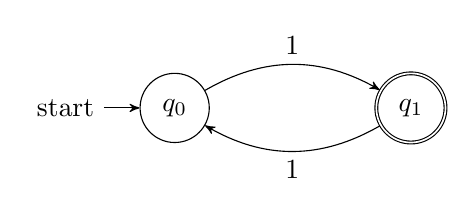
\begin{tikzpicture}
\node[state, initial] (q0) {$q_0$};
\node[state, accepting, right of=q0] (q1) {$q_1$};
\draw 
(q0) edge[bend left, above] node{1} (q1)
(q1) edge[bend left, below] node{1} (q0);
\end{tikzpicture}




\end{document}
